\documentclass{beamer}
\usepackage{graphicx}
\usepackage{geometry}
\geometry{left=1cm,right=1cm,top=1cm,bottom=1cm}

\usetheme[]{Antibes}
\useinnertheme[]{rounded}
\useoutertheme[]{tree}
\usecolortheme[]{crane}
\usefonttheme[]{}

\logo{
\includegraphics[height=1cm]{img/timg.jpeg}}

\title{my first beamer by \LaTeX}
\subtitle{this is what the subtitile looks like}
\author{panmeng}
\institute{ise}
\date{\today}
\titlepage

\begin{document}
    \begin{frame}
        \frametitle{This is the title page}
        \framesubtitle{and I want to see what framesubtitle looks like}
    \end{frame}

\section*{Outline}
    \begin{frame}{Outline}
        \tableofcontents
    \end{frame}

\section{Introducion}
    \begin{frame}
        \begin{theorem}
            theorem
        \end{theorem}

        \begin{corollary}
            corollary
        \end{corollary}

        \begin{block}{equation}
            \begin{equation}
                a^2 = b^2 + c^2
            \end{equation}
        \end{block}
    \end{frame}

\subsection{subsection}
    \begin{frame}
        subsection
        \begin{figure}
        %\centering
        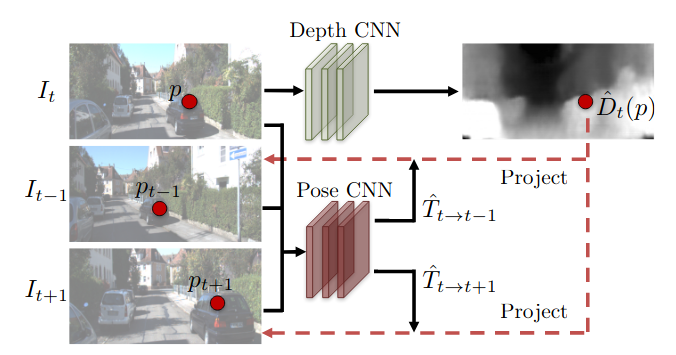
\includegraphics[height=3cm]{img/sfm.png}
        \caption{picture}
        \end{figure}
    \end{frame}
\subsection{subsection2}
    \begin{frame}
        subsection2
    \end{frame}
\section{Usage1}
    \begin{frame}
        Usage
    \end{frame}
\section{Usage2}
    \begin{frame}
        Usage
    \end{frame}
\section{Usage3}
    \begin{frame}
        Usage
    \end{frame}

\end{document}